\cite{\ref{}}\documentclass[10pt,a4paper]{book}
\usepackage[utf8]{inputenc}
\usepackage[english]{babel}
\usepackage{amsmath}
\usepackage{amsthm}
\usepackage{mathtools}
\usepackage{array}
\usepackage{booktabs}
\usepackage{gensymb}
\usepackage{slashed}
\usepackage{physics}
\usepackage{bbold}
\usepackage{stackengine}
\usepackage{amsfonts}
\usepackage{mathabx}
\usepackage[inkscapelatex=false]{svg}
\usepackage{amssymb}
\usepackage{graphicx}
\usepackage{geometry}
\usepackage{subcaption}
\usepackage{pdfpages}
\usepackage[numbers,sort&compress]{natbib}

\begin{document}

\chapter[Theory Introduction]{Everything you've ever wanted to know about particle physics and more}

In the beginning, there was nothing. Then, there was 

\begin{equation}
\begin{split}
\mathcal{L}_{SM}=& -\frac{1}{4}F_{\mu\nu}F^{\mu\nu}\\ +& i\overline{\psi}D\psi + h.c.\\ +& \overline{\psi}_i y_ij \psi_j \phi + h.c.\\ +& |D_\mu \phi|^2 - V(\phi).
\end{split}
\label{SM Lagrangian}
\end{equation}
Now, before we get too far ahead of ourselves, let us take the time to understand \emph{where} Eq. \ref{SM Lagrangian}, known as the Standard Model Lagrangian, comes from and what it represents. This chapter will be dedicated to this endeavour.

\section{The Standard Model}

\subsection{A quick overview of the universe}

To make the next section more readable, we will quickly describe the phenomenology of the Standard Model. Some details will be left for the next chapter. 

The Standard Model of particle physics is our best description of nature at the moment. It categorises all particles, into two categories: fermions and bosons. 

Bosons are the force-carrying particles, responsible for mediating the strong (in the case of the gluon) and electroweak interactions (in the case of the $W^\pm$, $Z$ and photon). Notably, the $W$ and $Z$ bosons are \emph{massive}, leading to the short range of the electroweak interaction, whereas the other two are massless. 

There is also the Higgs boson, which arises from the spontaneous symmetry breaking of the electroweak force. Unlike the other bosons, it is not responsible for mediating a force, but for giving mass to the other particles of the Standard Model. More details will follow in Section \ref{ssb}.

Fermions compose the matter sector of the Standard Model. They are divided into three generations, each with the same quantum numbers, but differing in there masses. The fermions are further divided into quarks and leptons. The main differentiator between the two is that the former are the sole particles in the matter sector who can interact via the strong force. Free quarks cannot be found in nature, and they are always bound to other quarks via gluons. 

Figure \ref{sm particles} shows all fermions and bosons currently belonging to the Standard Model, along with properties such as spin, mass, charge, etc.

\begin{figure}
    \centering
    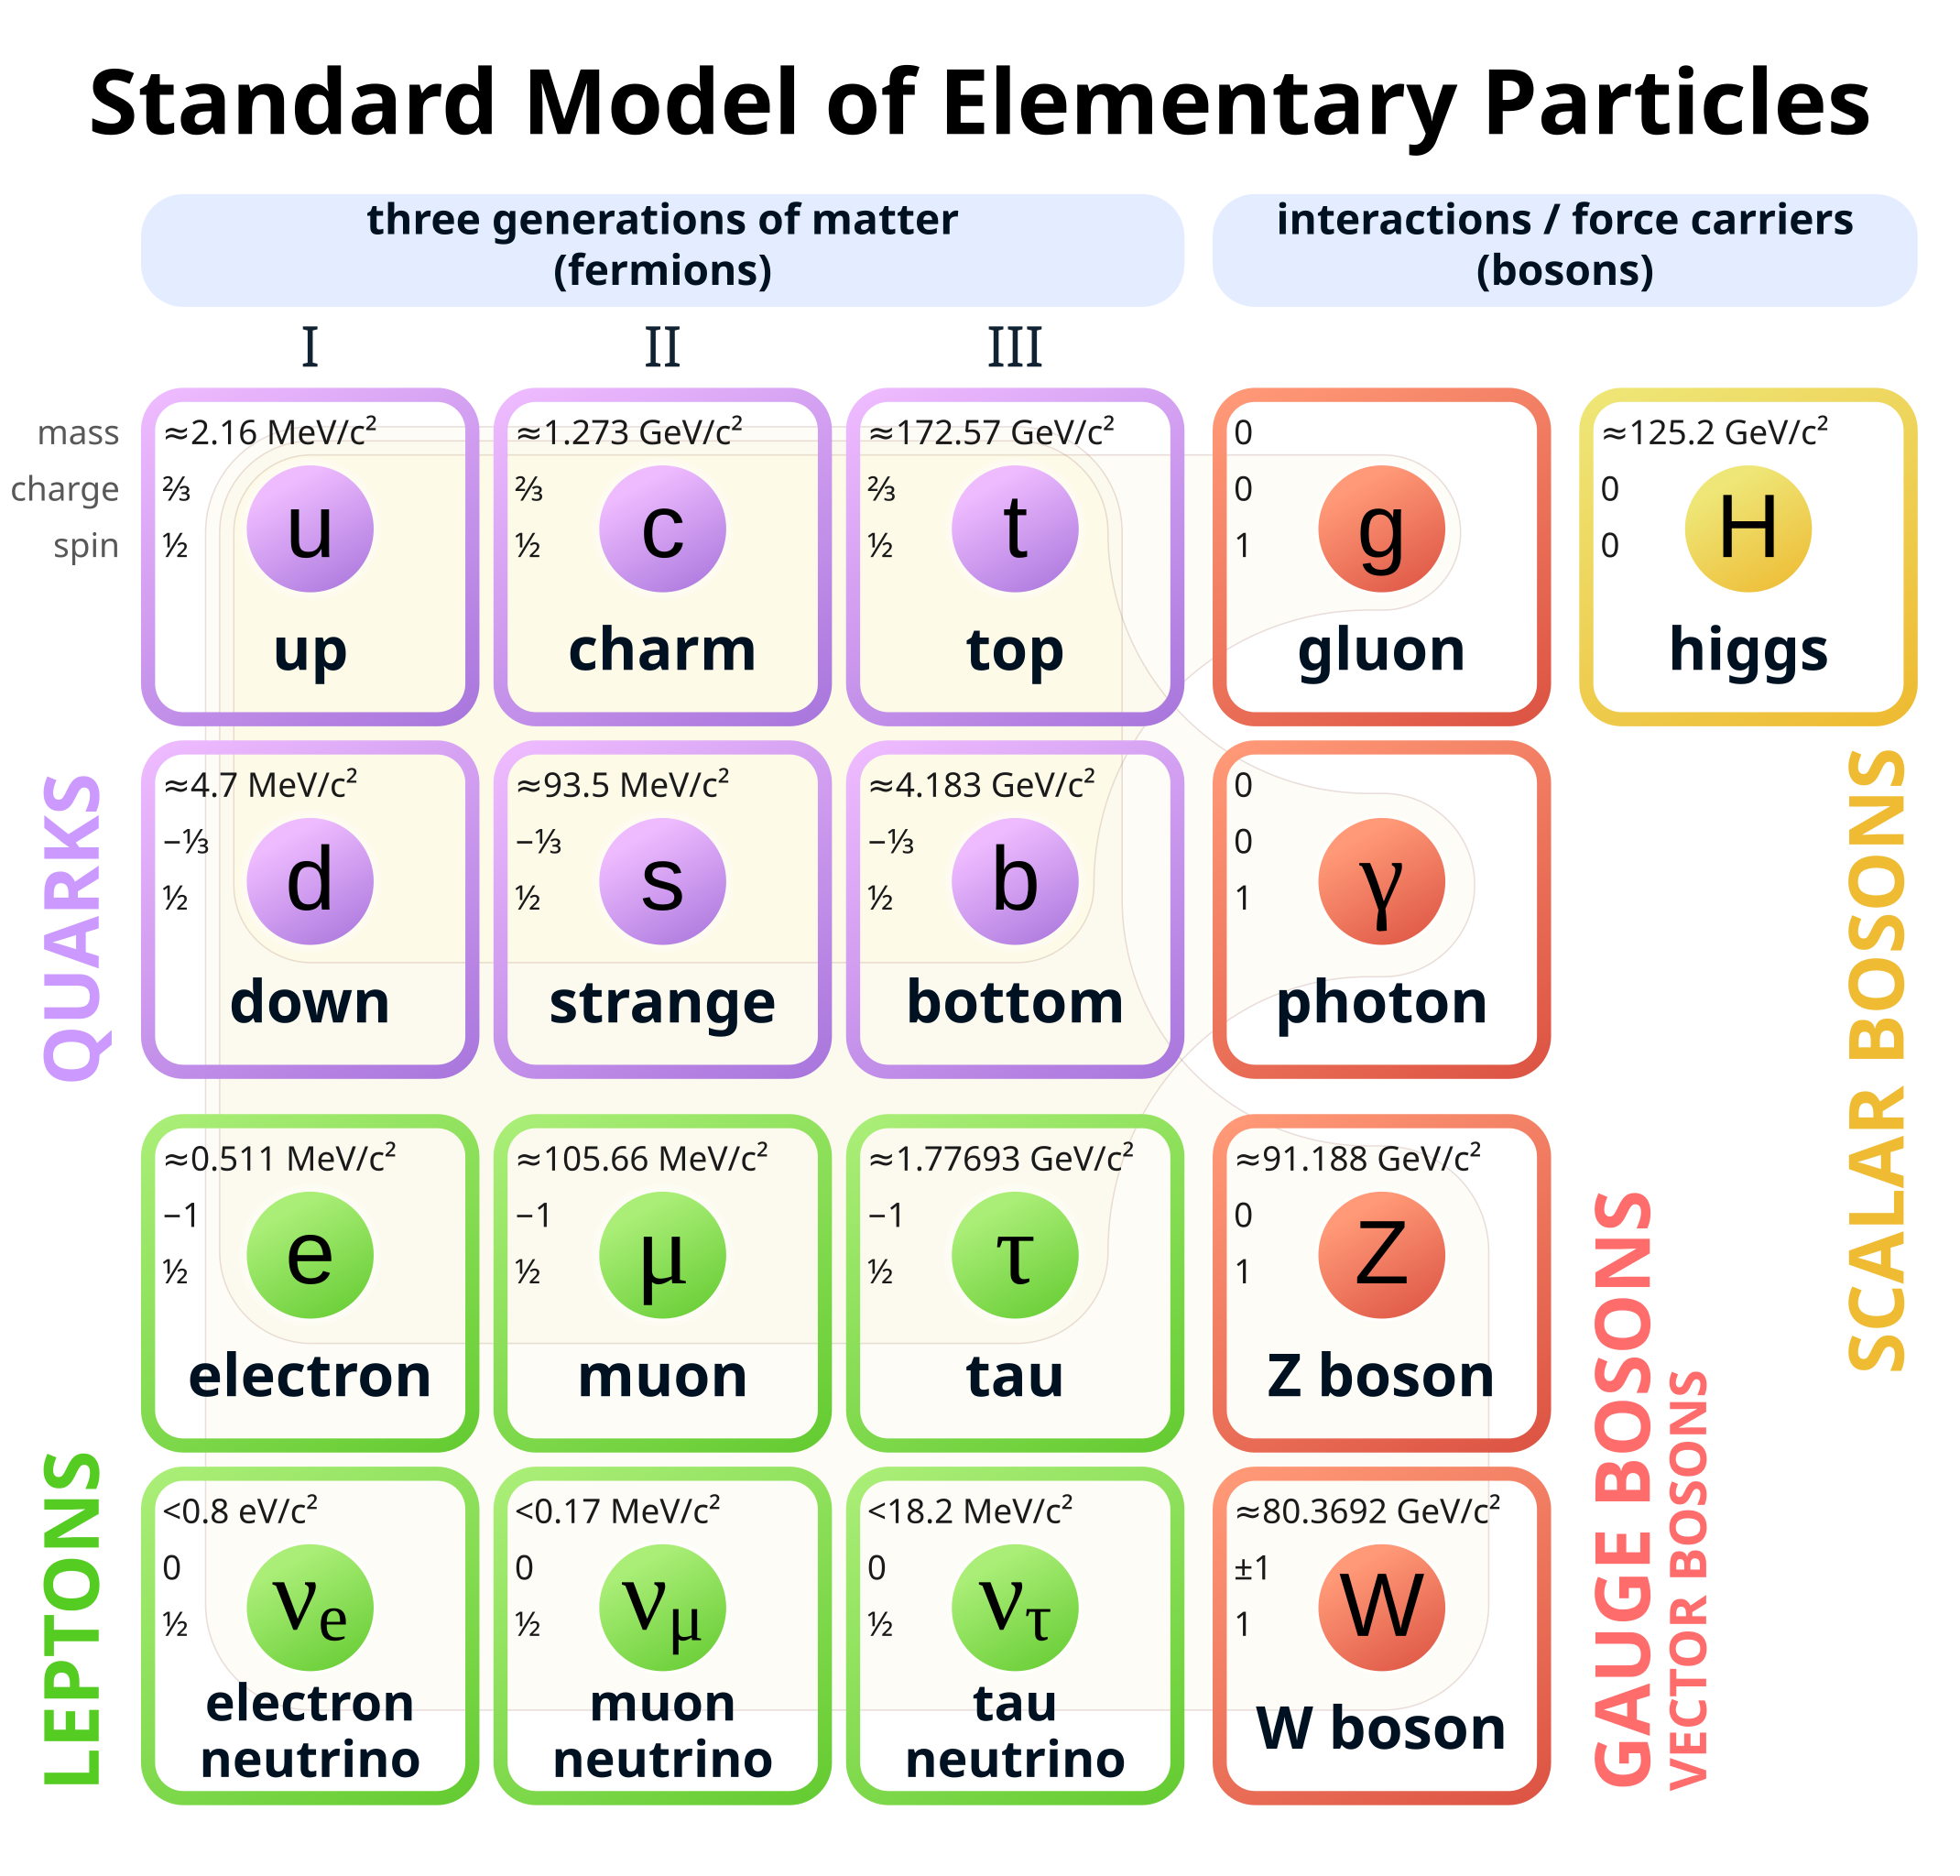
\includegraphics[width=0.75\linewidth]{theory chapter/Standard_Model_of_Elementary_Particles.png}
    \caption{Our current knowledge of the particles described by the Standard Model of particle physics \cite{wiki:sm}.}
    \label{sm particles}
\end{figure}

In the next section, we shall describe the Standard Model lagrangian in more detail. 

\subsection{The Standard Model for dummies}

The Standard Model Lagrangian $\mathcal{L}_{SM}$ (Eq. \ref{SM Lagrangian}) is invariant under local gauge symmetries of the group $SU(3)_C\otimes SU(2)_L \otimes U(1)_Y$. The three gauge groups which compose the tensor product each represent one of the fundamental symmetries underlying the forces of nature described by the Lagrangian, namely electromagnetism, the weak, and the strong interactions.

\subsubsection{Quantum electrodynamics}
The local $U(1)_{em}$ gauge symmetry leads to quantum electrodynamics (QED). This force describes interactions between charged particles and photons. Starting from a Dirac Lagrangian describing a free fermion
\begin{equation}
\mathcal{L}_D = \overline{\psi}(i\slashed{\partial} - m )\psi,
\label{Dirac}
\end{equation}

where $\psi$ is the fermion field, $\bar{\psi}$ its adjoint, $m$ the particle mass and $\slashed{\partial} = \partial_\mu \gamma^\mu$ the del operator, it is easy to see that $\mathcal{L}_D$ is invariant under global $U(1)_{em}$ transformations of the form $\psi^\prime = \exp(i\alpha)\psi$ when $\alpha$ is a constant. In fact, the adjoint operation on the $\psi^\prime$ field leads to a factor which cancels with the term $\exp(i\alpha)$.

In accordance with the gauge principle, let us now promote the global symmetry of the Lagrangian to a local one:
\begin{equation}
    \psi^\prime = \exp(ie\alpha(x))\psi
\label{local qed}
\end{equation}
where $\alpha$ is now a function which depends on the spacetime coordinates $x$ and $e$ is a constant representing the elementary charge. We can therefore define the covariant derivative
\begin{equation}
    D_\mu \dot{=} \partial_\mu + ieA_\mu
\end{equation}
where $A_\mu$ is the gauge (photon) field, and require that the term $\D_\mu\psi$ transform as $\psi$ itself would

\begin{equation}
    (D_\mu\psi) \rightarrow (D_\mu\psi)^\prime = \{\partial_\mu + ieA_\mu^\prime\}\psi^\prime = [\exp(ie\alpha(x))]D_\mu\psi.
\end{equation}

For the Lagrangian to remain invariant, $A^\prime_\mu$ must equal the following expression:
\begin{equation}
    A^\prime_\mu = A_\mu - \partial_\mu\alpha(x).
\end{equation}
We can then build a term to describe the free propagation of $A_\mu$ by computing the commutator of the covariant derivate
\begin{equation}
    [D_\mu, D_\nu] = ie\{\partial_\mu A - \partial_\nu A) \equiv ieF_{\mu\nu}
\end{equation}
where $F_{\mu\nu}$ is a tensor of the field $A_\mu$ defined from the commutator, i.e.
\begin{equation}
    F_{\mu\nu} = -\frac{i}{e}[D_\mu, D_\nu]
\end{equation}
In this way, we have all the ingredients needed to construct the QED Lagrangian

\begin{equation}
    \mathcal{L}_{QED} = -\frac{1}{4}F_{\mu\nu}F^{\mu\nu} + \overline{\psi}(i\slashed{D} - m )\psi - e\bar{\psi}\gamma^\mu\psiA_\mu.
\label{QED Lagrangian}
\end{equation}

The first term in \ref{QED Lagrangian} represents the kinetic term which describes the free propagation of the photon field and the central term is the Dirac Lagrangrian from which we started, with the del operator replaced by the covariant derivative to ensure invariance under the local gauge symmetry \ref{local qed}.

We would like to note that the method described is not the only way in which the QED Lagrangian (or that of any other fundamental force) can be derived. The principle advantage of the gauge protocol is that is does not assume any prior knowledge of the field $A_\mu$, and thus allows for the derivation of the gauge field in a general way. We know from classical electrodynamics, however, that $A_\mu$ represents the electromagnetic potential. One could thus use this prior knowledge to derive \ref{QED Lagrangian} by means of the minimal coupling. This procedure accounts for the electromagnetic potential in the four-momentum of the fermion, leading to a modification of Eq. \ref{Dirac} as follows
\begin{equation}
    \mathcal{L} = \overline{\psi}(i\slashed{\partial} - e\slashed{A} - m )\psi.
\end{equation}
One can then develop the additional terms of the Lagrangian, impose the local $U(1)_{em}$ gauge symmetry, and derive the necessary transformation of the field $A_\mu$ needed to respect the symmetry.

\subsubsection{QCD}
\label{QCD}
In a similar fashion, it is possible to derive the Lagrangian for strong interactions. In this case, we consider the spinor $q_f$

\begin{equation}
    q_f = \begin{bmatrix}
        q_f^1 \\
        q_f^2 \\
        q_f^3
    \end{bmatrix}
\end{equation}
where the subscript $f$ indicates quark flavour and the superscript is the colour index.
The free Lagrangian for these fields
\begin{equation}
    \mathcal{L}_D = \sum_f\overline{q}_f\left(i\slashed{\partial} - m_f\right)q_f
\end{equation}
is invariant under the transformation

\begin{equation}
    q_f \rightarrow q_f^\prime = \exp[i\theta_a\frac{\lambda^a}{2}]q_f
\end{equation}
where $\lambda_a$ is the generator of the $SU(3)$ symmetry group and $\theta_a$ is the parameter relative to the generator $\lambda_a$. In the fundamental representation, $SU(3)$ has eight generators, known as the Gell-Mann matrices, corresponding to the eight colour combinations ascribed to gluons. Gluons thus carry two colours, and a gluon exchange corresponds to an interaction which alters the colour of the quarks involved.

If we define the covariant derivative as before and promote the symmetry to a global one and follow through with the gauge protocol, we find that

\begin{equation}
    \mathcal{L}_{QCD} = -\frac{1}{4}G^a_{\mu\nu}G^{\mu\nu}_a + \sum_f\overline{q}_f\left(i\slashed{D} - m_f\right)q_f.
\end{equation}

as in the case for QED. There is one important difference, however: the $SU(3)$ symmetry group, unlike the $U(1)$ group, is non-abelian. A direct consequence of this fact is the self-coupling of the gluon, namely the 3- and 4-point gluon self-interaction, as can be seen from

\begin{equation}
    G^a_\mu \rightarrow (G^a_\mu)^\prime = G^a_\mu - \frac{1}{g_s}\partial_\mu\theta^a(x) - f^{abc}\partial_\mu\theta_b(x)G_{\mu c}.
\end{equation}

where $g_s$ is the coupling constant for the strong interaction and $f^{abc}$ the \emph{structure constant} of $SU(3)$, defined as 

\begin{equation}
    \left[\frac{\lambda_a}{2}, \, \frac{\lambda_b}{2}\right] = if_{abc}\frac{\lambda_c}{2}. 
\end{equation}

\subsubsection{Electroweak Unification} 

One can na\"{i}vely attempt to follow the gauge protocol to derive a Lagrangian describing weak interactions. The transformation acts on a weak-isospin doublet
\begin{equation}
    \psi_L = \begin{pmatrix}
  \nu_\ell \\ 
  \ell^-
\end{pmatrix}
\label{weak doublet}
\end{equation}

composed of the left-handed states of any two fermions belonging to the same generation (the right-handed state $\ell^+_R$ lives as a singlet). For the sake of simplicity, we have considered a charged lepton and neutrino. 

We can apply the the local gauge transformations
\begin{gather}
    \label{su2 transformation}
    \psi_L \rightarrow \psi_L^\prime = \exp[i\frac{\tau_j}{2}\alpha^j(x)]\psi \\
    \ell_R^+ \rightarrow \ell_R^{+\prime} = \ell_R^+
\end{gather}
where the matrices $\tau_j$ are the generators of the $SU(2)$ gauge group and $\alpha^j(x)$ represents the function which introduces local spacetime dependence to the transformation.

After following the gauge protocol, one can derive the gauge fields $W^1_\mu$, $W^2_\mu$ and $W^3_\mu$. Linear combinations of $W^1_\mu$ and $W^2_\mu$ are able to correctly describe charged current interactions attributed to the $W^\pm$ bosons

\begin{equation}
    W^\pm_\mu =    \frac{1}{\sqrt{2}}(W^1_\mu \mp i W^2_\mu)
    \label{Wpm}
\end{equation}
although $W^3_\mu$ \emph{is not} able to describe the neutral current as this field would only couple to left-handed fermions, and it is known from experiment that the neutral current couples to both left-handed and right-handed fermions.

To reconcile this fact, we can attempt to include electromagnetic interactions together with our description of the weak force. At first glance, this might seem counterintuitive, but considering that the photon is is the only other neutral boson available in the standard model besides the $Z$ boson, it makes sense to try to derive both the $Z$ boson and the photon from a linear combination of the neutral fields. The gauge group to consider is thus $SU(2)_L \otimes U(1)_Y$.

Let us introduce a quantity known as \emph{hypercharge}
\begin{equation}
    Y = 2(Q - I_3)
\end{equation}
where $Q$ represents electric charge and $I_3$ the weak isospin. $Y$ is defined in such a way that it distinguishes components of the weak isospin doublet in \ref{weak doublet} from right-handed states. For completeness, note that
\begin{gather}
    Y(\nu_\ell) = -1 \\
    Y(\ell^-) = -1\\
    Y(\ell^+) = -2.
\end{gather}

The full transformation under the new gauge group becomes
\begin{gather}
\label{electroweak gauge transformations}
\psi_L \rightarrow \psi_L^\prime = \exp\left[iy_1\beta(x)\right]\exp\left[i\frac{\tau_j}{2} \alpha^j (x)\right]\psi_L \\
\ell_R \rightarrow \ell_R^\prime = \exp\left[iy_2\beta(x)\right]\ell_R
\end{gather}
where $y_1$ represents the value of hypercharge for the left-handed states and $y_2$ for the right-handed states.
The covariant derivatives become

\begin{gather}
\label{EW covariant}
D_\mu \psi_L(x) = \left[\partial_\mu + ig\frac{\tau_j}{2}W^j_\mu(x) + ig^\prime \frac{y_1}{2} B_\mu(x) \right]\psi_L(x) \\
D_\mu \ell_R = \left[\partial_\mu ig^\prime \frac{y_2}{2} B_\mu(x)\right]\ell_R(x)
\end{gather}
where $g$ and $g^\prime$ are the two coupling constants for the left- and right-handed states. In general, these can be different from one another.

From Eq. \ref{EW covariant}, it is clear that we now have four gauge fields, the three $W^j_\mu$ fields from before and $B_\mu$. The fields $W^1_\mu$ and $W^2_\mu$ combine as before in Eq. \ref{Wpm} to form the $W^\pm$ bosons; the $Z$ boson and photon must be obtained through an appropriate linear combination in the neutral sector.

We can consider a generic rotation by an angle $\theta_W$, known as the weak mixing angle
\begin{equation}
\label{mapping}
\begin{bmatrix}
\cos\theta_W & \sin\theta_W \\
-\sin\theta_W & \cos\theta_W
\end{bmatrix}
\begin{bmatrix}
B_\mu \\
W^3_\mu
\end{bmatrix} =
\begin{bmatrix}
A_\mu \\
Z_\mu
\end{bmatrix}
\end{equation}
 
The interaction Lagrangian for the neutral sector in terms of $Z^\mu$ and $A^\mu$ can be written as

\begin{equation}
\label{neutral current lagrangian}
\begin{aligned}
\mathcal{L}_{NC} &= \overline{\psi}\gamma_\mu\left\lbrace g \sin\theta_W \frac{\tau_3}{2} + g^\prime \cos\theta_W \frac{Y(\psi)}{2} \right\rbrace \psi A^\mu \\
&+\overline{\psi}\gamma_\mu \left\lbrace g\cos\theta_W \frac{\tau_3}{2}- g^\prime\sin\theta_W\frac{Y(\psi)}{2}\right\rbrace\psi Z^\mu.
\end{aligned}
\end{equation}

If we continue to assume as in Eq. \ref{weak doublet} to be dealing with a charged lepton and neutrino, we can compare the first term in Eq. \ref{neutral current lagrangian} to the interaction term in Eq. \ref{QED Lagrangian} to find that 

\begin{equation}
-e = g\sin\theta_W \frac{\tau_3}{2} + g^\prime \cos\theta_W \frac{Y(\psi_{e})}{2}
\end{equation}

or, after specifying $\tau_3$ and $Y(\psi_e)$

\begin{equation}
g\sin\theta_W = g^\prime \cos\theta_W = e.
\end{equation}

We have successfully found an expression relating the couplings $g$ and $g^\prime$ to the electric charge $e$ through the weak mixing angle. The weak mixing angle is a free parameter of the Standard Model, and can only be determined experimentally. At the mass of the $Z$ boson, $\sin^2\theta_W$ has been measured to be \cite{ParticleDataGroup:2024cfk}
\begin{equation}
    \sin^2\theta_W(M_Z) = 0.231 29(4) \pm 1.7 \times 10^{-4}
\end{equation}

From Eq. \ref{neutral current lagrangian}, we can also see that the coupling of the $Z$ boson corresponds to 
\begin{equation}
g_{Z\nu} = \frac{e}{\sin\theta_w\cos\theta_W}\{\frac{1}{2}\tau_3 - Q\sin^2\theta_W\}.
\label{z coupling}
\end{equation}
We must specify the terms in the matrix to derive the numerical value of the coupling. For $\nu_L$ it is straightforward to show that $g_Z = \frac{e}{2\sin\theta_W\cos\theta_W}$. For the lepton $\ell^-$, we must decompose the spinor $\psi$ into the left-handed and right-handed components by means of the projection operator $P_{L/R} = \frac{1}{2}(1\mp\gamma^5)$, and, accordingly, consider the projections of the matrix in \ref{z coupling}. When doing so, we find that 

\begin{gather}
    g_{Z\ell_L} = \frac{e}{2\sin\theta_W\cos\theta_W}[I_3(\ell_L)(1 + 4Q_\ell\sin^2\theta_W)] \\
    g_{Z\ell_R} = \frac{e}{2\sin\theta_W\cos\theta_W}[I_3(\ell_R)].
\end{gather}
where $I_3$ as before indicates the weak isospin and $Q_\ell$ is the charge of the lepton in question.

We correctly find that the coupling constant differs for left-handed and right-handed spinors. We can also note that, if we were to rewrite the second term of Eq. \ref{neutral current lagrangian}, the use of the projection operators would lead to the V-A structure we expect of the neutral current. We can therefore fully reproduce the phenomenology of the weak interaction.

\subsection{Spontaneous symmetry breaking}

\label{ssb}

The careful reader would have surely noticed that none of the Lagrangians considered in the previous section contain massive gauge fields. However, in nature we know that the $W^\pm$ and $Z$ bosons are massive. How do we reconcile this fact?

The solution is not as simple as adding in a mass term by hand \`{a} la Dirac\footnote{This is known in literature as the Proca action}. This is due to the fact that a mass term of this form, i.e.

\begin{equation}
    \mathcal{L} = -\frac{1}{4}F^{\mu\nu}F_{\mu\nu} - m^2A^\mu A_\mu
\end{equation}
violates gauge symmetry. A more elegant solution is thus required.

Brout, Englert and Higgs found this solution for us, which earned Higgs the Nobel Prize in 2012.
The mechanism, aptly known as the Brout-Englert-Higgs (BEH) Mechanism, introduces a scalar field (the Higgs field) to the Standard Model and a potential (the Higgs potential) to induce spontaneous breaking of the $SU(2)\otimes U(1)$ gauge symmetry (SSB), leading to the mass of the gauge bosons.

%\begin{figure}
%    \centering
%    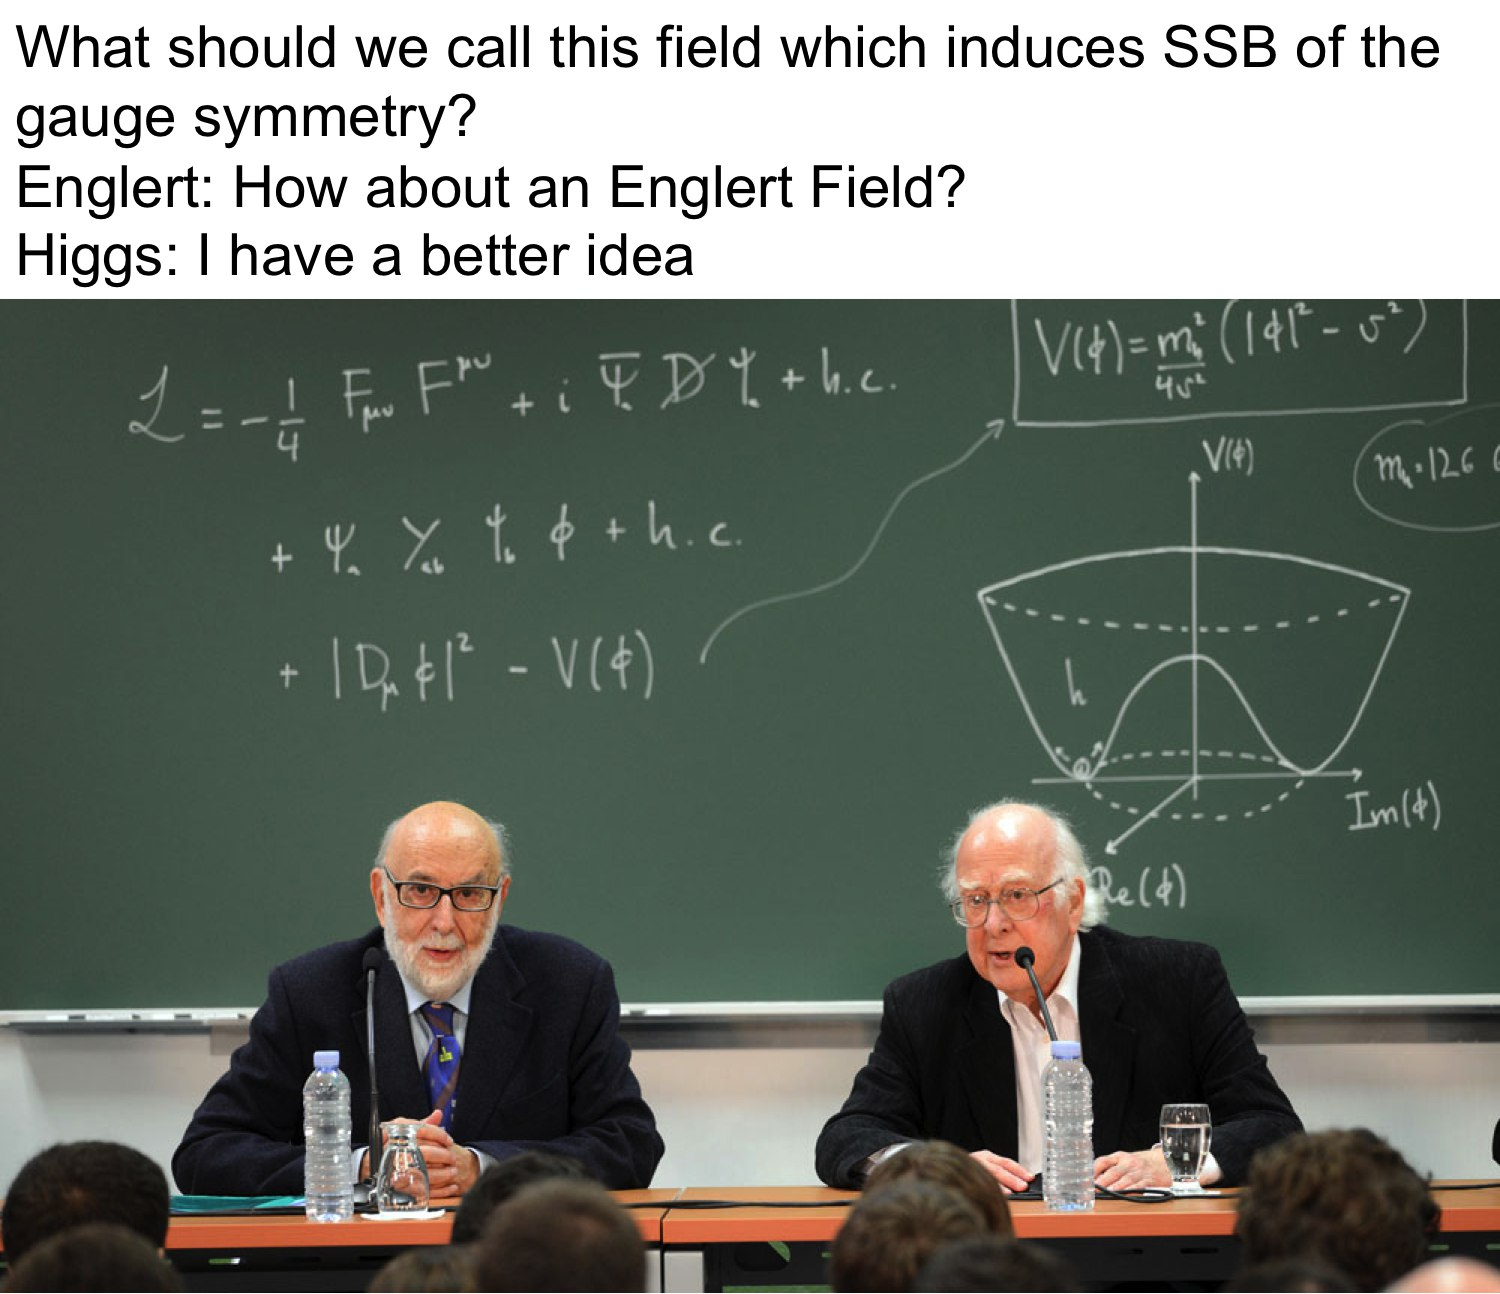
\includegraphics[width=0.5\linewidth]{beh_meme}
%    \caption{A satirical meme highlighting the fact that only one of the individuals involved with the discovery of the BEH Mechanism received the honour of having the field named after him.}
%    \label{fig:enter-label}
%\end{figure}

The BEH Mechanism is based on a Lagrangian of the form

\begin{equation}
    \mathcal{L} = (\partial_\mu\phi)^\dagger(\partial^\mu\phi) - V(\phi, \phi^\dagger)
    \label{higgs lagrangian}
\end{equation}
with the potential $V$ defined as

\begin{equation}
    V(\phi, \phi^\dagger) = \frac{\mu^2}{2}\phi^\dagger \phi - \frac{\lambda}{4}(\phi^\dagger\phi)^2.
\end{equation}
Here, $\phi$ is an $SU(2)$ doublet composed of two complex scalar fields

\begin{equation}
    \phi(x) = 
\begin{bmatrix}
\phi^+ \\
\phi^0
\end{bmatrix} =
\begin{bmatrix}
\frac{1}{\sqrt{2}}(\phi_3 + i\phi_4) \\
\frac{1}{\sqrt{2}}(\phi_1 + i\phi_2)
\end{bmatrix}
\label{higgs doublet}
\end{equation}
$m$ is the mass of the field $\phi$ and $\lambda$ is a free parameter. 

Note that the Lagrangian in Eq. \ref{higgs lagrangian} is invariant under the $SU(2)\otimes U(1)$ gauge symmetry.

We can minimise the potential to find the ground state of $\phi$

\begin{equation}
    \frac{\partial V}{\partial \vert \phi \vert} = \mu^2\vert \phi \vert + \lambda\vert\phi\vert^3 .
\end{equation}

If $\lambda, \mu^2 > 0$, the only minimum is for $\phi = 0$. Instead, if $\mu^2 < 0$, there is a maximum at $\phi = 0$ and an infinite set of degenerate minimum states found at $\bra 0\phi^\dagger\phi \ket 0 = -\sqrt{m^2/\lambda} \equiv v$. This quantity is known as the \emph{vacuum expectation value}.

We can choose \emph{ad libitum} any one of these states to define our ground state, say

\begin{equation}
    \phi_0 = \frac{1}{\sqrt{2}}\begin{bmatrix}
    0 \\
     v
    \end{bmatrix}.
\end{equation}

It is easy to show that, although the Lagrangian in Eq. \ref{higgs lagrangian} remains invariant under the $SU(2) \otimes U(1)$, \emph{the ground state does not respect the same symmetry!} Specifically, it is the action of the generators $\tau^i$ and $y$ from Eq. \ref{electroweak gauge transformations} which lead to a variation of the field. 

We would now like to find a way to give mass to the $W^\pm$ and $Z$ bosons, while leaving the photon massless. The Goldstone theorem teaches us that for each broken generator, there exists a corresponding massless particle. Na\"{i}vely, we have just stated that there are in fact \emph{four} broken generators. This problem is quickly resolved through a linear combination

\begin{gather}
    Q = \frac{1}{2}\tau_3 - \frac{1}{2}y \\
    Q^\prime =  \frac{1}{2}\tau_3 + \frac{1}{2}y.
\end{gather}
Now, $Q$ is unbroken while $\tau_1, \tau_2$ and $Q^\prime$ remain broken. The corresponding massless particles are not physical, but are said to be ``eaten'' by the gauge bosons, giving rise to their mass. 

Considering small perturbations of the vacuum state $\phi_0$

\begin{equation}
    \phi (x) = \frac{1}{\sqrt{2}}\exp\left[\frac{i\tau_j\xi_j(x)}{2} \right]\begin{bmatrix}
0 \\
v + H(x)
\end{bmatrix}
\end{equation}
where $\xi_j(x)$ is the a parameter dependent on the spacetime coordinates and $H(x)$ is a small perturbation the field $\phi^0$ from Eq. \ref{higgs doublet}, corresponding to the Higgs boson. The exponential term can be gauged away

\begin{equation}
    \phi (x) \rightarrow \phi^\prime (x) = \exp\left[-\frac{iT_j\xi_j(x)}{2} \right]\phi.
\end{equation}

Now, we can follow through with the gauge protocol and consider the term

\begin{equation}
(D_\mu\phi)^\dagger(D_\mu\phi) = \frac{g^2}{4}\left(v^2 + 2vH + H^2\right)W^+_\mu W^{- \mu} + \frac{1}{8}(v + H)^2 \left( g^2 W^3_\mu W^{3\mu} - 2gg^\prime W^3_\mu B^\mu + g^{\prime 2}B_\mu B^\mu \right).
\end{equation}
Here, it is easy to read off all the information that we've sought from the start: the mass of the $W^\pm$ is found to be $m_W^2 = \frac{1}{4}g^2v^2$, that of the $Z$ boson (after electroweak unification) is $M_Z = \frac{1}{4}v^2(g^2+g^{\prime 2}$, and the photon field $A_\mu$ remains massless. Moreover, we find no interaction term between the $H$ and $A_\mu$ and we find that the coupling of the Higgs boson and gauge bosons is, as expected, proportional to the square of their masses. We have thus solved the problem of massive gauge bosons in the Standard Model.

\subsection{Fermion Masses}

Unfortunately, also fermion mass terms fail to respect the gauge symmetry of the Standard Model Lagrangian. Specifically, since the $SU(2)_L$ symmetry acts differently on left-handed and right-handed spinors, terms of the form $m\bar{\psi}\psi$ are clearly not invariant after decomposition into their respective components. 

Once again, the Higgs field can solve this problem. Let us once again consider transformations of the type in Eq. \ref{su2 transformation}. When applied to the Higgs field $\phi$, we find that, to first order

\begin{equation}
    \phi \rightarrow \phi^\prime = \exp[ig\frac{\tau_j}{2}\alpha^j(x)]\phi \approx [1 + ig\frac{\tau_j}{2}\alpha^j(x)]\phi.
\end{equation}

Likewise, the same transformation on the field $\bar{\psi}_L$ leads to
\begin{equation}
    \bar{\psi}_L \rightarrow \overline{(\psi_L)^\prime} = \bar{\psi}_L\exp[ig\frac{\tau_j}{2}\alpha^j(x)] \approx \bar{\psi}_L[1 - ig\frac{\tau_j}{2}\alpha^j(x)].
\end{equation}

The quantity $\bar{\psi}_L\phi$ is therefore invariant under this transformation. The same holds true if we consider $\bar{\psi}_L\phi\psi_R$, as $\psi_R$ does not transform under $SU(2)_L$.

We can thus write the Yukawa Lagrangian

\begin{equation}
    \mathcal{L}_Y = -k(\bar{\psi}_L\phi\psi_R + \bar{\psi}_R\bar{\phi}\psi_L)
    \label{yukawa lagrangian}
\end{equation}

where $k$ is a coupling constant. Eq. \ref{yukawa lagrangian} respects the full gauge symmetry of the Standard Model Lagrangian, and gives mass to particles and antiparticles. We can specify the terms to some species of fermion $f$ to find that $m_f = k_fv/\sqrt{2}$, where $k_f$ is the Yukawa coupling for $f$. Note that the coupling is arbitrary and no fermion mass is explicitly predicted by the Standard Model.

\section{QCD}

The LHC is a hadron collider. This means that the dominant interaction is QCD. It therefore is worth taking the time to look more deeply into this fundamental force. We will start with a description of the internal structure of the proton and then move to the perturbative evolution of the final state, hadronisation, and jet formation. 

\subsection{Running of the coupling constant}

In Section \ref{QCD} we gave a brief overview of the gauge theory underlying QCD. Here, we would like to touch upon an aspect which we previously ignored: the running of the coupling constant. 

The strength of an given interaction governed by a given force is determined by the coupling constant. Despite the name, the coupling is anything but constant. Instead, it varies as a function of energy. 

This variation can be naively understood as the (anti-)``screening'' of a charge by the self-energy of the photon, gluon, or any other gauge boson. 

For QED, this explanation is intuitive: as one approaches a charge, there are fewer virtual electron-positron pairs which may screen this charge. In a scattering experiment, one can approach the charge by reaching higher and higher energies. Thus, as the photon energy increases, the value of the coupling increases.

More rigorously, the photon self-energy diverges and one needs \emph{renormalisation} to regularise this divergence. Sparing the details, the regularisation procedure relies on the fact that experimentally the electric charge (and thus the coupling) is measured to be finite. If we know the electric charge at some scale $q^2 = \mu^2$, where $q^2$ is the energy of the virtual photon, the one loop photon self-energy corrections $\Pi(q^2)$ and $\Pi(\mu^2)$ are both separately divergent. However, their difference

\begin{equation}
    \Pi(q^2) - \Pi(\mu^2) \approx \frac{1}{12\pi^2}\ln\left(\frac{q^2}{\mu^2}\right)
\end{equation}
is finite. 

This can be inserted into the expression for the coupling to give

\begin{equation}
\alpha(q^2) = \frac{\alpha(\mu^2)}{1 - \frac{\alpha(\mu^2)}{3\pi}\ln\left(\frac{q^2}{\mu^2}\right)}.    
\end{equation}

In QCD, things are complicated by the gluon self-interaction. This introduces additional contributions to the gluon self-energy which completely alters the behaviour. 

The analogous expression for $\alpha_S$ turns out to be

\begin{equation}
    \alpha_S = \frac{\alpha(\mu^2)}{1 + B\frac{\alpha_S(\mu^2)}{3\pi}\ln\left(\frac{q^2}{\mu^2}\right)}
\label{qcd running}
\end{equation}

where $B$ is a quantity which depends on the the number of fermionic and bosonic loops which are relevant to the calculation. The general expression depends on the number of quark flavours $N_f$ and the number of colours $N_c$

\begin{equation}
    B = \frac{11N_c - 2N_f}{12\pi}.
\end{equation}

The behaviour of the coupling constant fundamentally depends on the number of flavours and colours. In our universe, at relevant energy scales, $B > 0$ leading to an \emph{anti-screening} of the colour charge at high energies. This implies that \emph{QCD is only perturbative at high energies}, a property known as \emph{asymptotic freedom}. The scale at which this transition occurs is determined by the Landau pole $\Lambda \sim 300 $ MeV. 

Figure \ref{running} shows the running of the coupling constants for the electromagnetic, weak and strong interactions. 

\begin{figure}
    \centering
    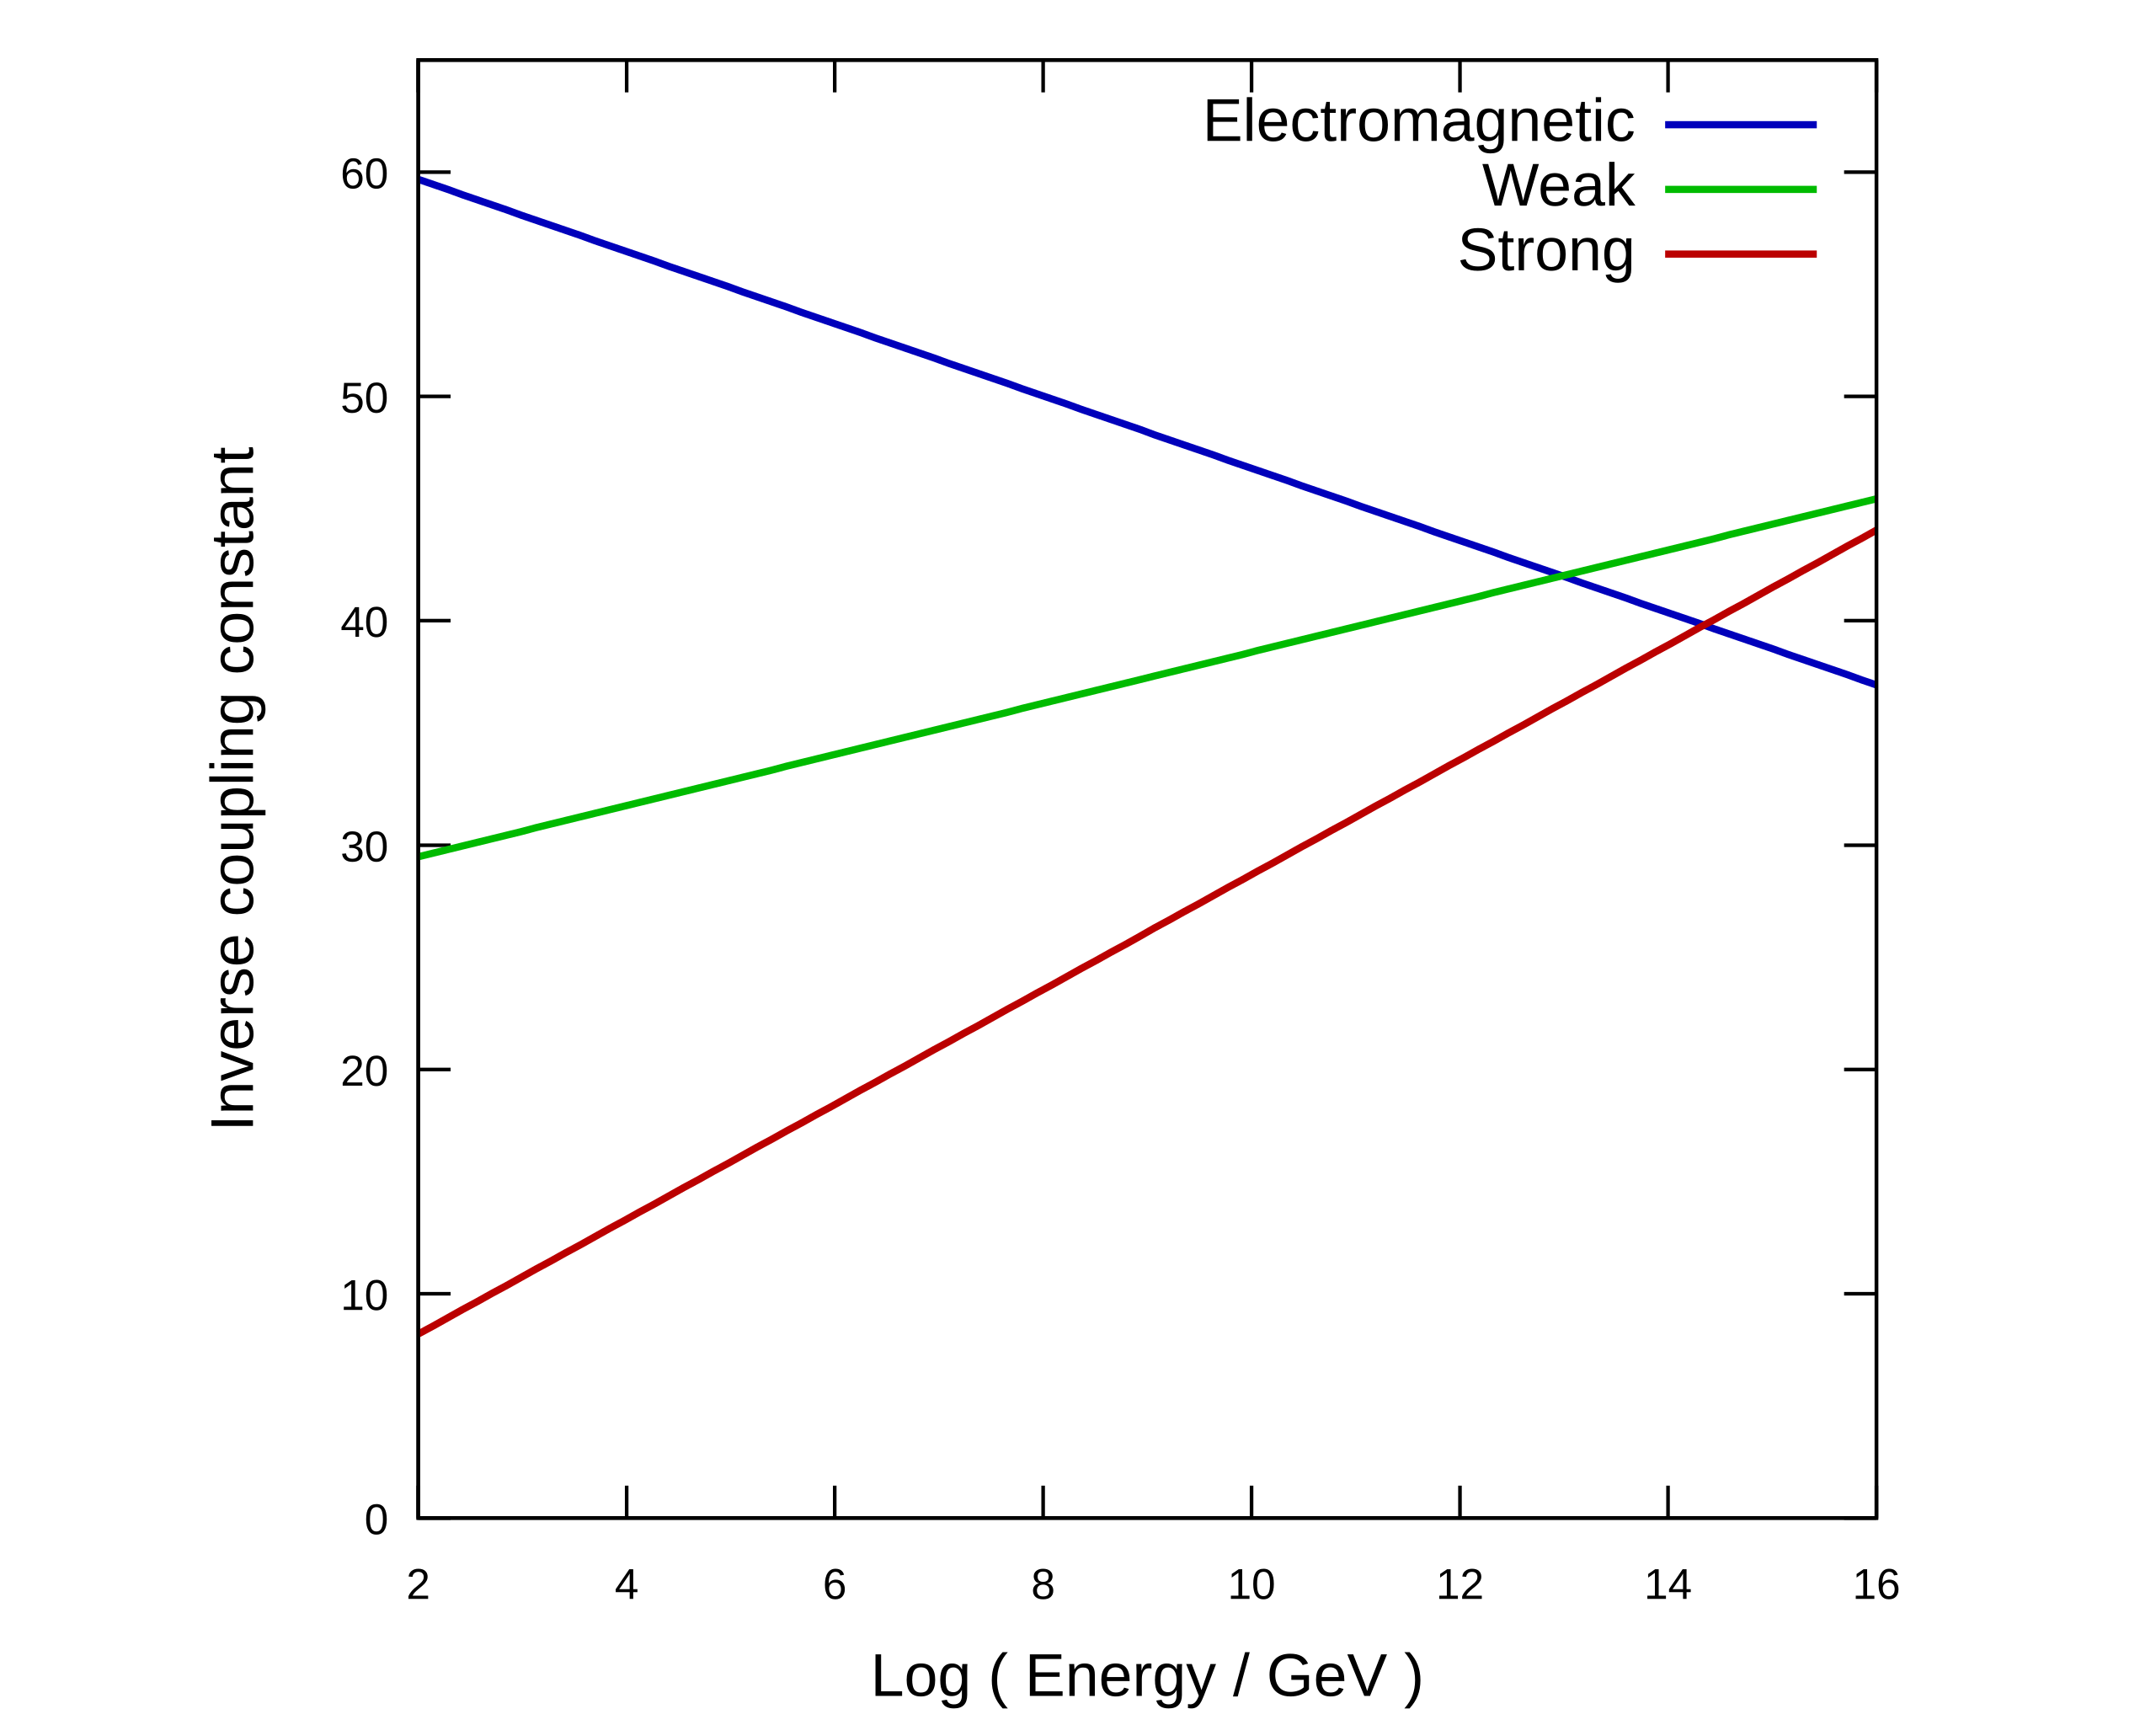
\includegraphics[width=0.75\linewidth]{theory chapter/Running_coupling_constants.png}
    \caption{The values of the coupling constants for the various forces described the Standard Model at different energy scales \cite{wiki:running}.}
    \label{running}
\end{figure}


\subsection{Parton distribution functions}
When protons collide at high energies, it is not the protons themselves which interact, but their constituents, known as partons. The proton is a dynamic system; its composition is described by \emph{parton distribution functions} (PDFs), $f_p(x,Q^2)$, which depends on both the fraction of momentum carried by the species of parton $p$ and the energy of the proton $Q^2$.

PDFs cannot be calculated. They must be extracted from data. This is done by reverse engineering the measured cross section to deconvolve the PDF contribution. Specifically, we can see this by looking at the ``master equation'' for calculating cross-sections in $pp$ collisions producing a final state $X$
\begin{equation}
    \sigma_{pp\rightarrow X} = \sum_{a,b} \int_0^1 dx_1 \int_0^1 dx_2 f_a(x_1, \mu_F)f_b(x_2,\mu_F)\int d\sigma_{ab \rightarrow X} (x_1P_1, x_2P_2, \mu_F, \mu_R).
\end{equation}
Here, the term $d\sigma_{ab\rightarrow X}$ is the differential cross section for some interaction involving partons $a$ and $b$ which produces the final state $X$. It depends on the momentum of the partons $p_{i} = x_{i}P_i$, given by the total momentum of the hadrons $P_i$ and the relative momentum fractions $x_i$, as well as the factorisation scale $\mu_F$ which sets the energy cut-off above which physics is described by the hard scattering and the renormalisation scale $\mu_R$ which establishes the reference energy at which to define the physical parameters. We must then take into account the probability of extracting the partons of flavour $a$ and $b$ with momenta $p_i$. This is where the PDFs $f_a$ and $f_b$ come into play. Lastly, the momentum fractions are integrated over all possible values, and a sum over all possible flavours is taken, ultimately leading to the cross section $\sigma_{pp\rightarrow X}$. 

Several collaborations actively fit PDFs using old and new data, taken from both the LHC as well as LEP, HERA, and other colliders. Some of the best data for PDF fits actually comes from Deep Inelastic Scattering experiments, where electrons, muons or neutrinos are used to probe the proton. The advantage in this case is the simpler form of the master equation, which contains only one PDF. 

Figure \ref{pdf} shows two such PDF fit carried out by the NNPDF collaboration at 10 GeV and $10^4$ GeV at next-to-next-to leading order (NNLO). Here, the order in perturbation theory refers to both the calculation of the hard process and the scale evolution of the PDF, which will be discussed in more detail in a later section.

\begin{figure}
    \centering
    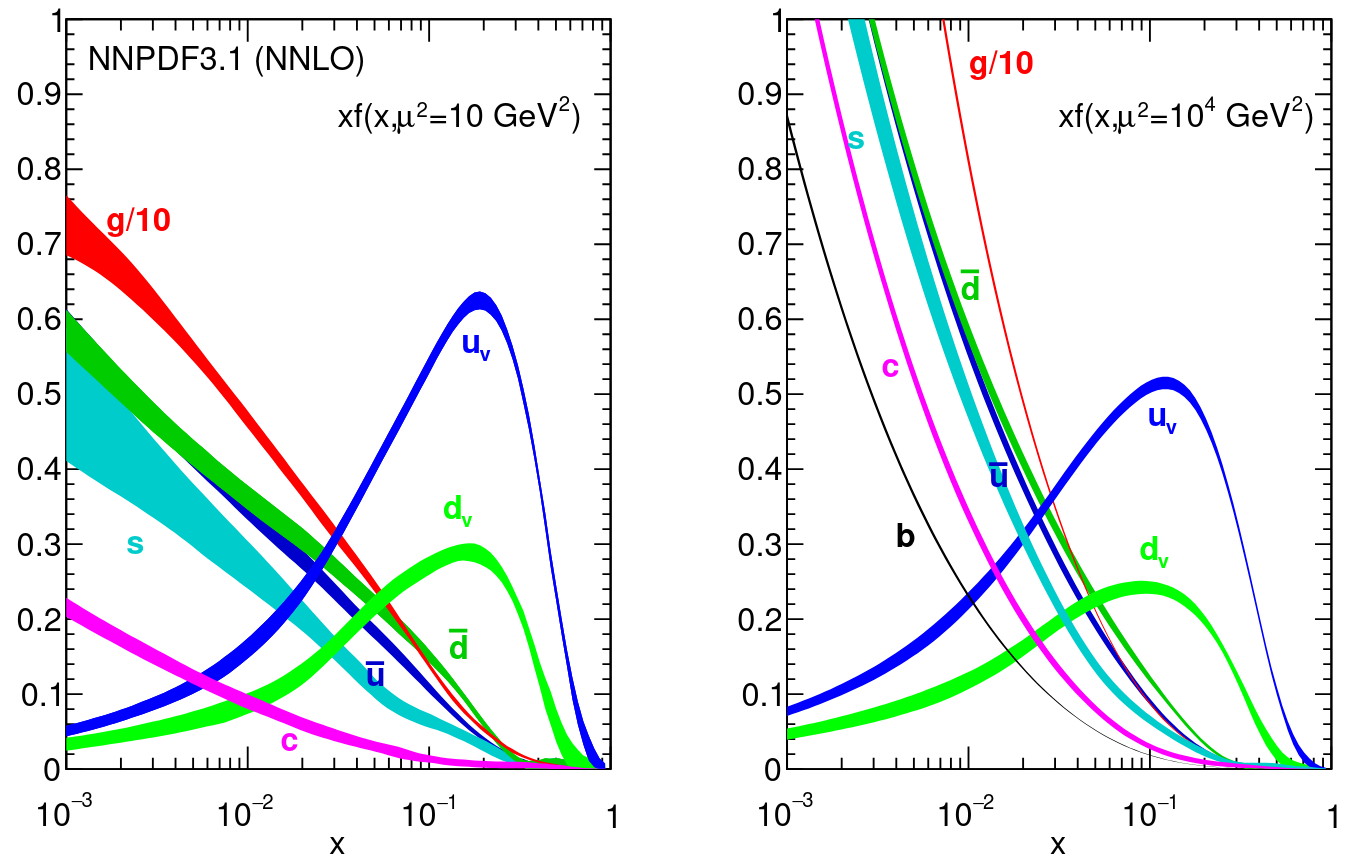
\includegraphics[width=0.9\linewidth]{nnpdf}
    \caption{The NNLO proton PDFs in the NNPDF3.1 fit for quarks and gluons at 10 GeV (left) and $10^4$ GeV (right) \cite{NNPDF:2017mvq}.}
    \label{pdf}
\end{figure}

\subsection{Final state evolution}
Partons in the final state are typically produced off-shell by the hard-scattering process and need a way to shed their virtuality. This is done through the parton shower. If we consider the radiation of a gluon subsequent to the production of a $q\bar{q}$ pair, we find that

\begin{equation}
    \frac{d\sigma_{q\bar{q}g}}{d\cos\theta dz} \approx \sigma_{q\bar{q}}C_F\frac{\alpha_S}{2\pi}\frac{2}{\sin^2\theta}\frac{1 + (1 - z)^2}{z}
    \label{divergence}
\end{equation}
which is proportional to the cross-section for the $q\bar{q}$ production process, the colour-factor $C_F = (N_C^2 -1)/2N_c$, the strong coupling $\alpha_S = g_s^2/4\pi$, and the energy fraction of the gluon $z$.

From here, it is already clear that the expression diverges in two circumstances:  soft and collinear gluon emissions. A final state quark is thus very likely to emit a gluon which is either soft, collinear, or both. 

The term $C_F\frac{1 + (1-z)^2}{z}$ in Eq. \ref{divergence} is known as the \emph{splitting function} $P_{gq}$, which, in this case, can be interpreted as the probability of finding quark emitting a collinear gluon with momentum fraction $z$. Analogous splitting functions exist for other types of emissions, 

\begin{gather}
    P_{qq}(z) = C_F \frac{1 + z^2}{1 - z} \\
    P_{gg}(z) = C_A \frac{z^4 + 1 + (1 - z^4)^2}{z(1-z)} \\
    P_{pg} = T_R(z^2 + (1 - z)^2)
\end{gather}

where $C_A = N_C$ is the gluon colour factor and $T_R$ is a colour factor fixed to $1/2$ by convention. These splitting functions are all reported at leading order.

The splitting functions also describe any initial-state radiation that may be in the event. In this case, they appear in the Dokshitzer-Gribov-Lipatov-Altarelli-Parisi (DGLAP) equations, used to calculate the evolution of PDFs to a different energy scale. The evolution of quark PDFs is goverened by

\begin{equation}
    \frac{dq_f(x, Q^2)}{d\log Q^2} = \frac{\alpha_S}{2\pi}\int_x^1 \frac{dy}{y} \left[ q_f(y, Q^2)P_{qq}\left(\frac{x}{y}\right) + g(y, Q^2)P_{qg}\left(\frac{x}{y}\right) \right]
\end{equation}

where $g_y$ is the gluon PDF, whereas the evolution of the gluon PDF is goverened by

\begin{equation}
    \frac{dg(x,Q^2)}{d\log Q^2} = \frac{\alpha_s}{2\pi}\int_x^1 \, \frac{dy}{y} \left[\sum_f q_f(y,Q^2)P_{gq}\left(\frac{x}{y} \right) + g(y,Q^2)P_{gg}\left(\frac{x}{y} \right) \right].
\end{equation}
The DGLAP equations are what allow us to measure PDFs at a given energy scale and evolve them to different values of $Q^2$, eliminating the need to scan in variables other than $x$.

\subsection{Hadronisation}

The parton shower describes the perturbative QCD evolution of the final state, down to about $\sim1$ GeV. At lower energies, due to the running of the coupling constant $\alpha_S$, the physics becomes non-perturbative and hadronisation occurs.

Hadronisation is the process of hadron formation from the quarks in the final state. We know from experimental observation that free quarks do not exist in nature and that only $SU(3)$ colour singlet states are observed. This fact is known as \emph{colour confinement}. 

As it is an inherintly non-perturbative process, there is only a heuristic understanding of the formation of hadrons. The explanation is based on the gluon-gluon self-interaction. As two quarks in a $q\bar{q}$ pair are pulled apart, they exchange virtual gluons. The colour field is confined to a tube between the two quarks. This tube is uniform and characterised by a constant energy density, leading to a linear potential $V(r) \sim \kappa r$, where $\kappa$ is a constant roughly equal to the size of a hadron, i.e. $\kappa \sim 1$ GeV/fm. 

As the potential is linear, the energy in the field increases as the distance between the quarks $r$ increases. At some point, this leads to the production of a new $q^\prime\bar{q}^\prime$ pair from the vacuum. This splits the colour flux tube in two. This process repeats, leading to the production of $n$ hadrons by the creation of $n-1$ new $q_i\bar{q}_i$ pairs. 

This picture of hadronisation forms the basis of the Lund string model used by Monte Carlo generators. Another model, the cluster model, describes the same physics but through a different lens. 

\subsection{Jets}

It is feasible to calculate cross-section for exclusive (or semi-inclusive) production of some hadrons in the final state. To do so, one needs to consider Fragmentation Functions $D_f(z)$, or the probability of a quark of flavour $f$ will hadronise into a hadron of species $D$ with fraction $z$ of the total energy available. Like PDFs, Fragmentation Functions must be determined from data and cannot be calculated from first principles due to their non-perturbative nature.

It is impractical, however, to explicitly calculate final states with more than just a few hadrons. There are just too many hadrons present in the final state, and, more importantly, it is experimentally impossible to explicitly determine the exact species of each hadron. 

The solution to this problem is jets. Broadly speaking, jets are an agglomeration of particles roughly produced in the same direction. They can be defined at multiple levels: at parton level, jets are defined using the particles produced in the hard process and parton shower; at hadron level, jets are defined from the hadrons obtained after modelling hadronisation. Experimentally, jets are defined based on tracks and calorimeter clusters in a given event.

\subsubsection{Jet algorithms}
To actually be useful, jets need to be defined more rigorously than just a broad concept of a cone containing particles which are close together\footnote{This was literally the first concept of a jet}. Today, the most widely used algorithms \emph{sequential recombination algorithms}, where nearby particles are combined based on some criteria to build a jet. 

\paragraph{$k_t$ algorithms}

In most cases, the an algorithm from the family of $k_t$ algorithms is used to define a jet. These algorithms are based on a set of distances

\begin{equation}
\begin{cases}
d_{ij} = \min(k_{ti}^{2p}, k_{tj}^{2p})\frac{\Delta_{ij}^2}{R^2} \\
d_{iB} = k_{ti}^{2p}.
\end{cases}
\end{equation}

Here, $d_{ij}$ is the distance between two particles $i$ and $j$, with $p_T$ $k_{ti}$ and $k_{tj}$, respectively. $\Delta^2 = (y_i - y_j)^2 + (\phi_i - \phi_j)^2$ is the distance between the two particles in the $y-\phi$ plane, while $p$ and $R$ are parameters, with $R$ representing the radius of the jet we wish to cluster. $d_{iB}$, on the other hand, represents the \emph{beam distance}, and is a reference condition used by the algorithm.

The condition for clustering two particles together is as follows: if $d_{ij} < d_{iB}$, the particles $i$ and $j$ are clustered together, and they are combined according to some \emph{recombination scheme}. The most commonly used recombination scheme for jets produced by hadron colliders is the $E$-scheme, where the four-momenta are simply added $p_i + p_j  = p_{ij}$. Another notable scheme is the Winner-Takes-All or WTA-scheme, where the four-momentum of the particle with the highest $p_T$ of the two to be combined is assigned to the jet. 

The parameter $p$ can take any value, though 3 cases are notable enough to deserve mention:
\begin{itemize}
    \item $p = 1$, also known as the $k_t$ algorithm
    \item $p = 0$, the Cambridge-Aachen (C/A) algorithm
    \item $p = -1$, or the anti-$k_t$ algorithm.
\end{itemize}
By varying $p$, the momentum-dependent weight on the distance $d_{ij}$ varies, modifying the algorithm accordingly. The most common choice nowadays is the anti-$k_t$ algorithm. This is because it is the algorithm which most matches the definition of a jet, i.e. it is the most conic as can be seen in Figure \ref{jet shapes}. The reason for this shape, however, is the $1/k_t^2$ weight applied to the distances. In fact, this weight causes soft particles to be clustered with nearby hard particles, rather than together as would occur in the case of the $k_t$ algorithm. This property is known as \emph{soft resilience.}

\begin{figure}
    \centering
    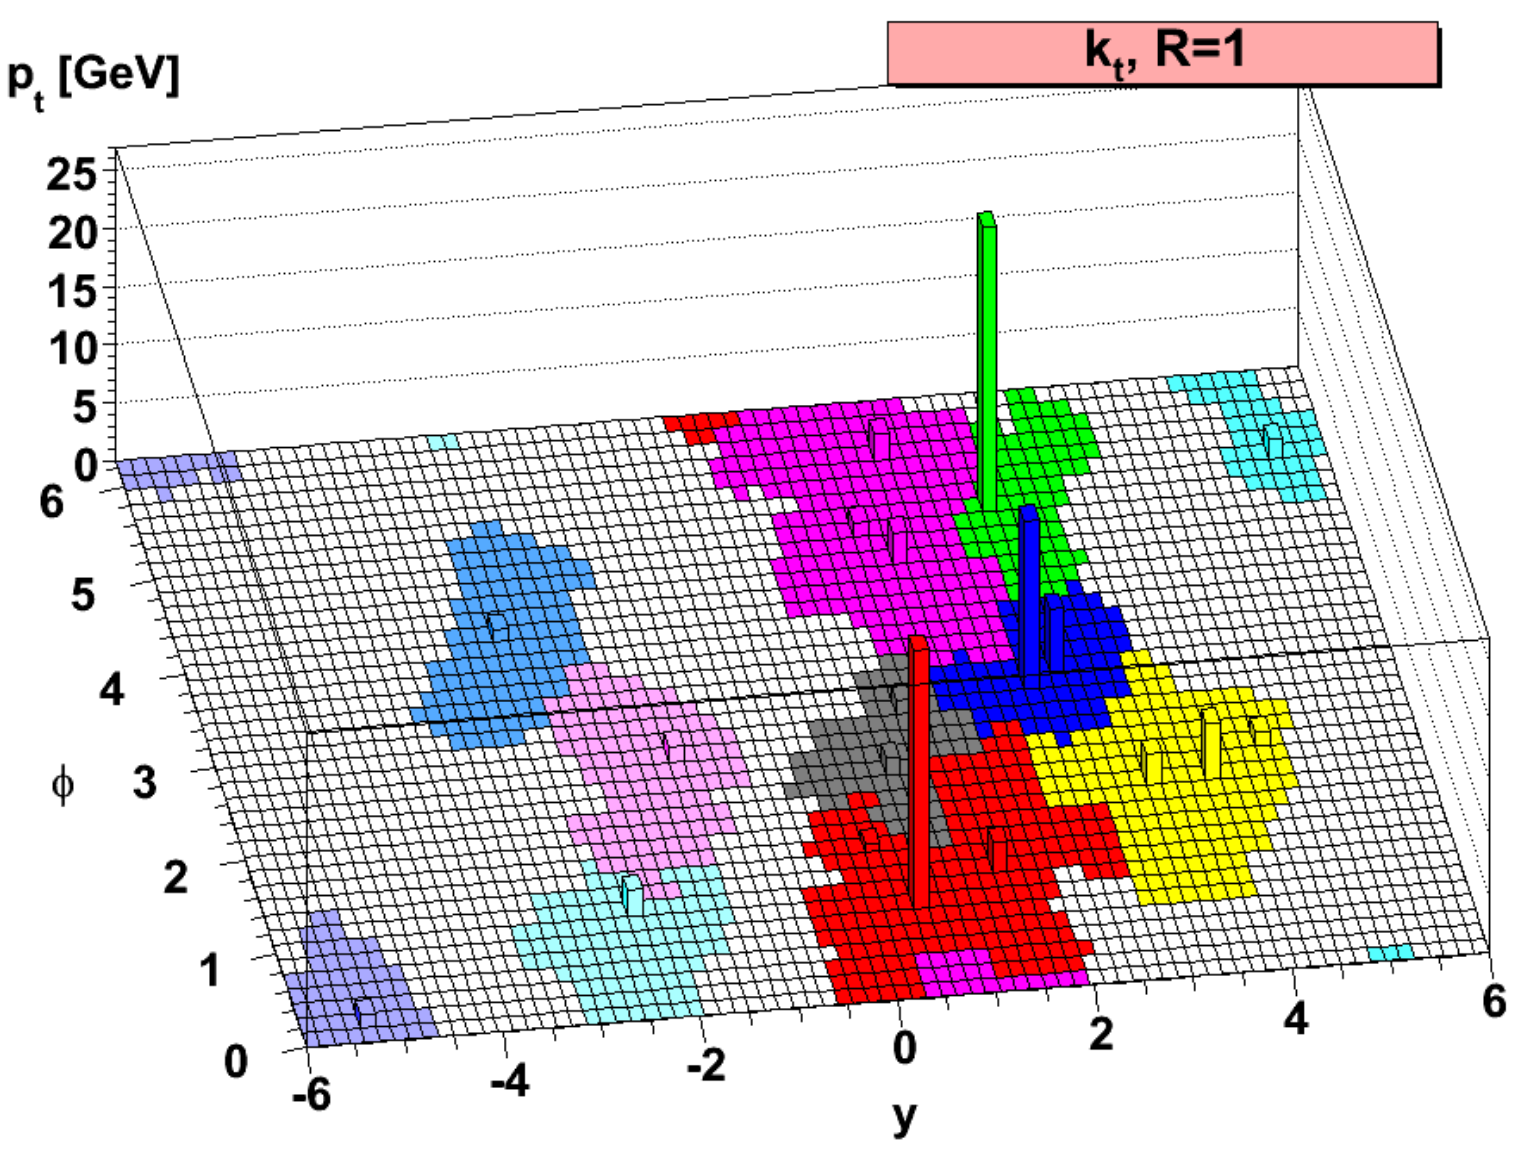
\includegraphics[width=0.49\linewidth]{theory chapter/kt.png}
    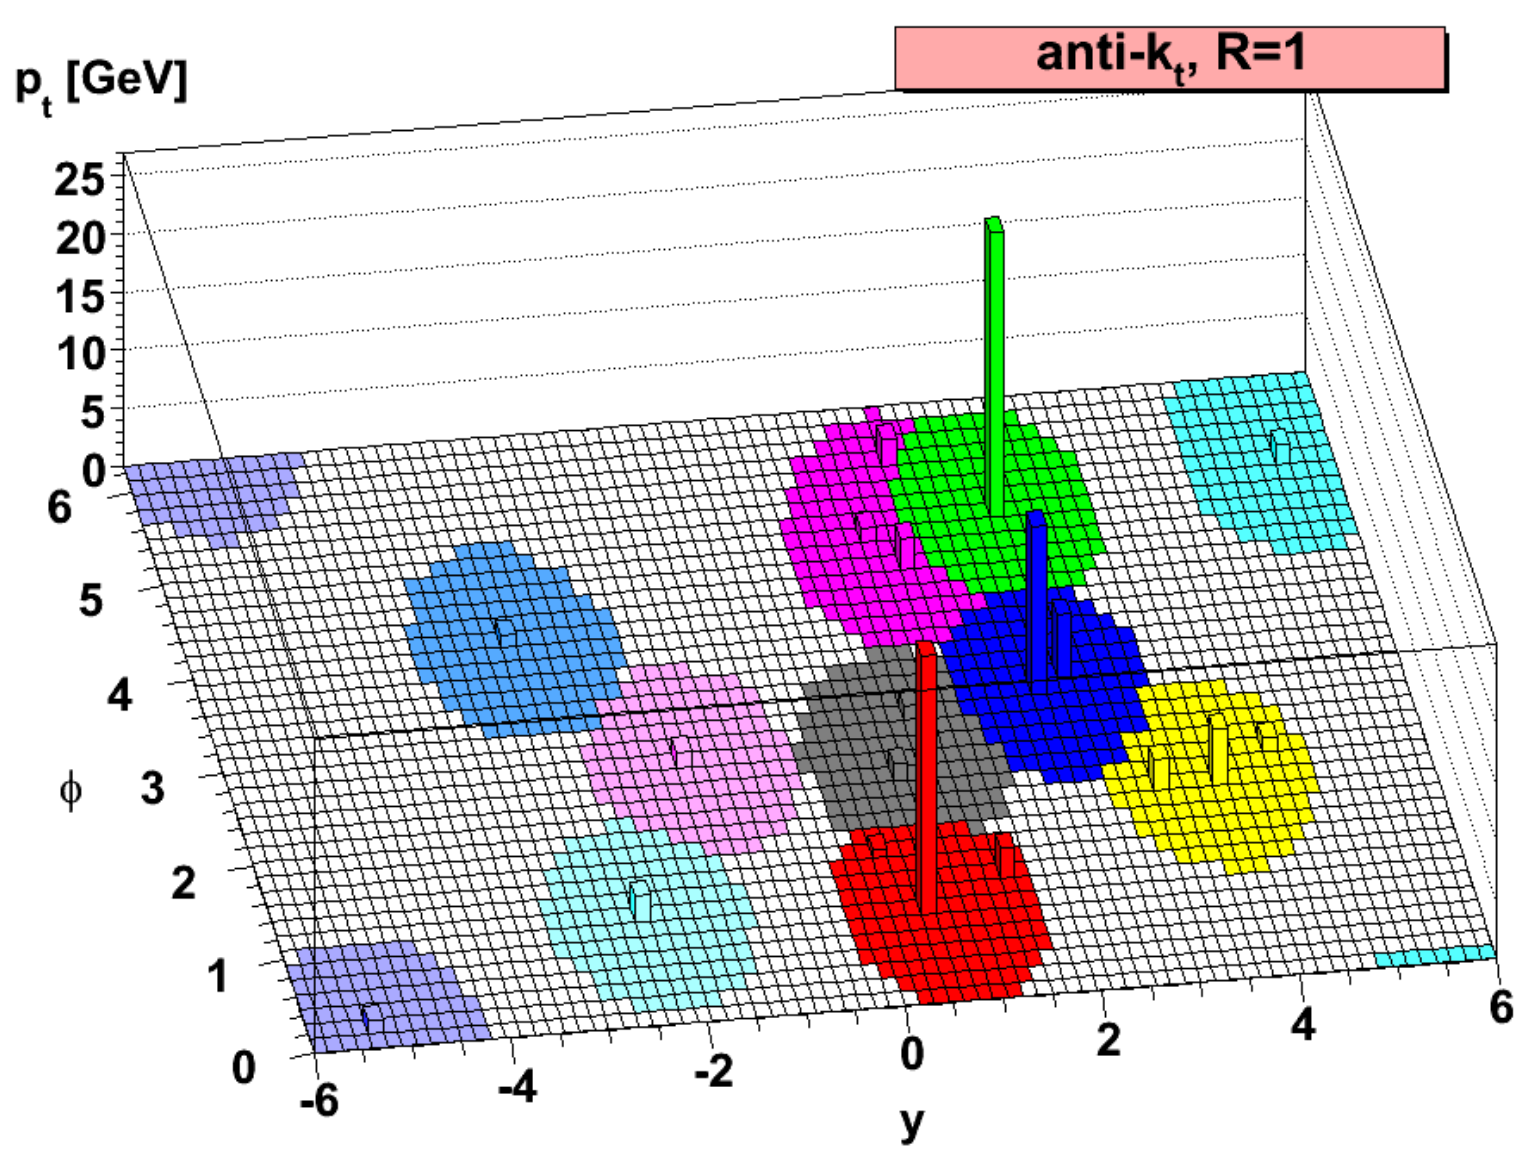
\includegraphics[width=0.49\linewidth]{theory chapter/anti-kt.png}

    \caption{The jet shape for jets clustered with the $k_t$ algorithm (left) vs. for those clustered with the anti-$k_t$ algorithm (right) \cite{Cacciari:2008gp}.}
    \label{jet shapes}
\end{figure}

\subsection{Jets and IRC safety}
An important property for jets to maintain is infrared and collinear (IRC) safety. Namely, this means that ideally a jet is defined in such a way that 
it is insensitive to soft and collinear radiation.

Consider once again Eq. \ref{divergence}. Gluons radiated during the parton shower tend to be soft and collinear due to the presence of the divergences. Jets are, by design, meant to contain the radiation off of a hard parton. It is therefore desirable that a given algorithm behaves in this way.

Mathematically, this property translates to the condition
\begin{gather}
\mathcal{O}(X; p_1, \dots, p_n, p_{n+1} \rightarrow 0) \rightarrow  \mathcal{O}(X; p_1, \dots, p_n ) \label{IRC safety}\\
\mathcal{O}(X; p_1, \dots, p_n \parallel p_{n+1}) \rightarrow \mathcal{O}(X; p_1, \dots, p_n+p_{n+1}).
\label{collinear safety}
\end{gather}

Eq. \ref{IRC safety} states that if a particle $p_{n+1}$ is emitted with four-momentum tending to 0, then the jet function $\mathcal{O}$ behaves as if this particle were not present. Likewise, Eq. \ref{collinear safety} states that if the particle $p_{n+1}$ is emitted collinear to the particle $p_n$, then the jet algorithm treats these as one particle with momentum $p_n+p_{n+1}$. 

The good news is that the $k_t$ algorithms in use today \emph{are} in fact IRC safe. This is a major factor as to why the algorithm is as widespread as it is. Other aspects, such as IRC safe flavour association, is not yet so common. We will touch upon this in Chapter 3 (\textcolor{red}{add reference}).

\subsubsection{Jet substructure}
Once we have defined our jets based on some algorithm, it is interesting to study the internal structure of these jets. This field of study is known as \emph{jet substructure}.

Jet substructure is a burgeoning field which has its roots in the start of the LHC programme. The aim of the field is to understand the radiation pattern within jets. This is directly tied to the origin of said jets, as jets originating from a top quark, for example, will have a different structure from those originating from a $Z$ boson, for example. This is illustrated in Figure \ref{jss}.

\begin{figure}
    \centering
    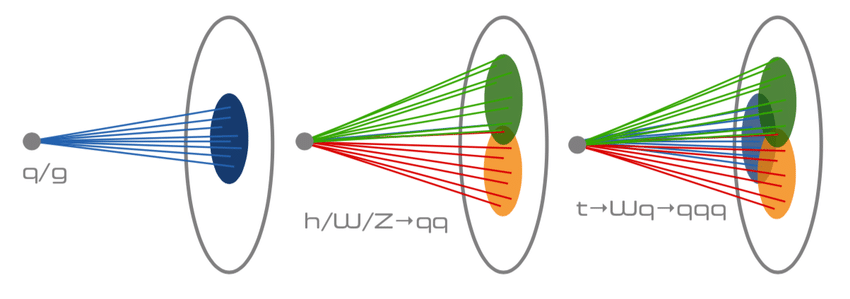
\includegraphics[width=0.9\linewidth]{jets}
    \caption{An illustration of the substructure of jets originating from quarks/gluons, $W/Z/H$ bosons, and top quarks \cite{JEDI}.}
    \label{jss}
\end{figure}

The simplest jet substructure observable is the jet mass, defined as
\begin{equation}
    m^2 = \left(\sum_i k_i\right)^2,
\end{equation}
where the sum runs over all particles $i$ with momenta $k_i$ in the jet. Other examples include the jet thrust, $N$-subjettiness, and the Lund Jet Plane. We will discuss more about this last observable in Section \textcolor{red}{add link}.

\subsection{Jet grooming}
To aid in the study of jet substructure, it is often useful to \emph{groom} jets. Grooming is a technique by which jets are cleaned of soft radiation, which may have its origins from particles other than the seed of the jet. It leaves intact the jet core, allowing for more accurate predictions to be made. 

One notable example of a grooming algorithm is the SoftDrop algorithm. It works by reclustering a given jet with the C/A algorithm, in order to obtain the angular-ordered clustering history (emissions) of the jet. Starting from the softest branch, the algorithm grooms away soft emissions until the following condition is met

\begin{equation}
    \frac{\min(p_{ti}, p_{tj})}{p_{ti} + p_{tj}} = z_{\text{cut}}\left(\frac{\Delta R_{ij}}{R}\right)^\beta
\end{equation}
where $p_{ti}$ and $p_{tj}$ refer to the $p_t$ of the subjets $i$ and $j$, respectively, $\Delta R_{ij}$ is the distance between the two in the rapidity-$\phi$ plane. $z_\text{cut}$ and $\beta$ are a parameters which regulate the emissions to be cut, with $z$ holding the usual meaning of $p_{ti}/(p_{ti} + p_{tj})$. If the removal condition is never satisfied, the jet can either be removed or left as is.

Another notable grooming technique is known as \emph{trimming}~\cite{Krohn:2009th}. Trimming involves reclustering a jet's constituents into jets of smaller radius. If the $p_t$ fraction carried by one of these smaller-radius jets is below a certain threshold, i.e. 5\%, it and all its constituents are removed. The remaining constituents are clustered back into a jet of the original radius.

\subsection{Heavy flavour jets}

Jet substructure can give insight on the particle which gives origin to the jet. For instance, quark/gluon jet discrimination is possible due to the fact that gluon originated jets will have a higher particle multiplicity due to the large colour factor and more wide-angle emissions.
Differences among quark-initiated jets are also possible, arising mainly from the presence of a heavy-flavour quark. If the seed particle has a significant mass, such as in the case of $c$-quarks and $b$-quarks, the mass scale intrinsically affects the evolution of the final state.

If we consider the probability of emitting a gluon carrying energy fraction $z$ at an angle $\theta^2$, the full expression with mass is found to be
\begin{equation}
    P(z,\theta^2)dzd\theta^2 = \frac{\alpha_sC_F}{2\pi}\frac{dz}{z}\frac{d\theta^2}{\theta^2 + \frac{m^2}{E^2}}.
\end{equation}
When $m\rightarrow 0$, we can read the soft and collinear divergences with which we are now familiar. Instead, if $m \not\approx 0$, we find that the collinear divergence is now \emph{shielded} by the mass effect. This is known as the \emph{dead cone effect}~\cite{Dokshitzer:1991fd} and it is illustrated in Figure~\ref{fig:deadcone}. The emission process is no longer scale invariant, and within a cone of angle $\theta_D^2 = m^2/E^2$, the emission of gluons is suppressed.

\begin{figure}
    \centering
    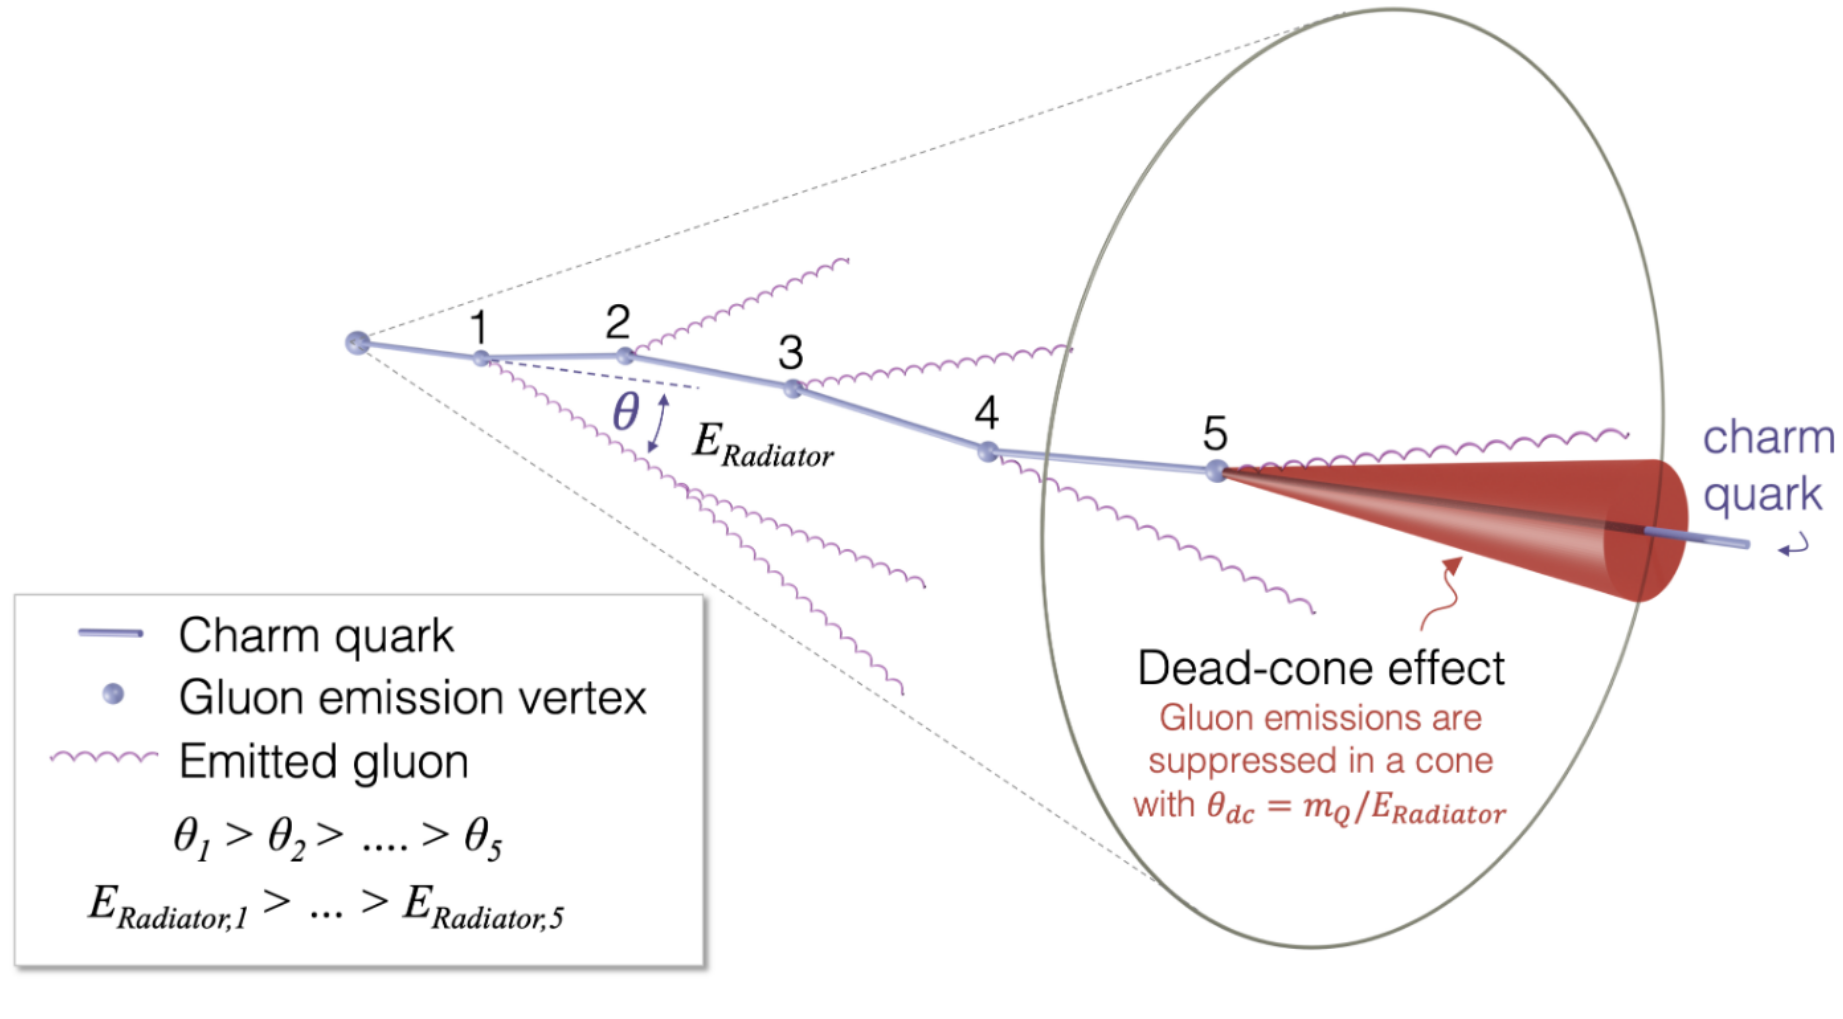
\includegraphics[width=0.75\linewidth]{theory chapter/deadCone.png}
    \caption{A schematic representation of the dead cone effect initiated by a charm quark~\cite{ALICE:2021aqk}.}
    \label{fig:deadcone}
\end{figure}

It is useful to note that, to first order, the dead cone can be equivalently seen as depending on $m/p_t$ ratio. This can be seen by writing the four-momenta of the quarks and gluon involved in the emission in terms of $(p_t, y, \phi, m)$. The dead cone condition predicting a suppression for $\theta \lesssim \theta_D$ thus becomes $\Delta R \lesssim m/p_t$, where the $p_t$ refers to that of the quark after emission.

\section*{Conclusions}
In this chapter, we gave a quick overview of the Standard Model of particle physics and the symmetries which underlie it. We then looked into the phenomenology of QCD and gave an introduction to jets and jet substructure, focusing especially on heavy flavour jets. In the next chapter, we will continue with our introduction, but from a more experimental perspective, focusing instead on the ATLAS detector and on object reconstruction.

\end{document}